\documentclass[11pt,a4paper]{article}
\usepackage[american]{babel}
\usepackage[utf8x]{inputenc}
\usepackage{url}
\usepackage{amsmath}
\usepackage{amsfonts}
\usepackage{graphicx}
\graphicspath{{images/}}
\usepackage{parskip}
\usepackage{fancyhdr}
\usepackage{wrapfig}
\usepackage{indentfirst}
\usepackage{vmargin}
\usepackage[font=small,labelfont=bf]{caption}
\usepackage[colorinlistoftodos]{todonotes}
\usepackage{indentfirst}
\usepackage{hyperref}
\usepackage{fullpage}
\usepackage{booktabs}
\usepackage{caption}
\usepackage{enumerate}
\usepackage{indentfirst}
\usepackage{color}
\usepackage{verbatim}
\usepackage{capt-of}
\usepackage[]{algorithm2e}
\usepackage{float}
\usepackage{multirow}
\usepackage{framed}
\usepackage{listings}
\usepackage{datetime}
\usepackage{url}
\usepackage[numbers]{natbib}
\usepackage{epstopdf}
\usepackage{subfig}
\usepackage{pdfpages}


\numberwithin{equation}{section}

\renewcommand{\vec}[1]{\mathbf{#1}}

 
\definecolor{codegreen}{rgb}{0,0.6,0}
\definecolor{codegray}{rgb}{0.5,0.5,0.5}
\definecolor{codepurple}{rgb}{0.58,0,0.82}
\definecolor{backcolour}{rgb}{0.95,0.95,0.92}
 
\lstdefinestyle{mystyle}{
    backgroundcolor=\color{backcolour}, 
    commentstyle=\color{codegreen},
    keywordstyle=\color{magenta},
    numberstyle=\tiny\color{codegray},
    stringstyle=\color{codepurple},
    basicstyle=\footnotesize,
    breakatwhitespace=false,         
    breaklines=true,                 
    captionpos=b,                    
    keepspaces=true,                 
    numbers=left,                    
    numbersep=5pt,                  
    showspaces=false,                
    showstringspaces=false,
    showtabs=false,                  
    tabsize=2
}
 
\lstset{style=mystyle}
\setmarginsrb{1.5 cm}{1.5 cm}{1.5 cm}{1.5 cm}{0.5 cm}{1 cm}{0.5 cm}{1 cm}

\title{Coursework 3 \\
Reinforcement Learning (CO-424H)}							% Title
\author{Adrian Löwenstein}								% Author
\date{\today}											% Date

\makeatletter
\let\thetitle\@title
\let\theauthor\@author
\let\thedate\@date
\makeatother


\pagestyle{fancy}
\fancyhf{}
\rhead{\theauthor}
\lhead{Reinforcement Learning}
\cfoot{\thepage}

\begin{document}

\maketitle

\section{Understanding of MDPs}
\paragraph{1)}
The trace generated by my CID (01594572) is $ \tau =  s_2 \ 1 \ s_0 \ 1 \ s_1 \ 0 \ s_2 \ 1 \ s_0 \ 1 \ s_2 \ 0 $
\paragraph{2)}
We can create the MDP graph displayed in figure \ref{CID}.
\begin{figure}[H]
	\centering
	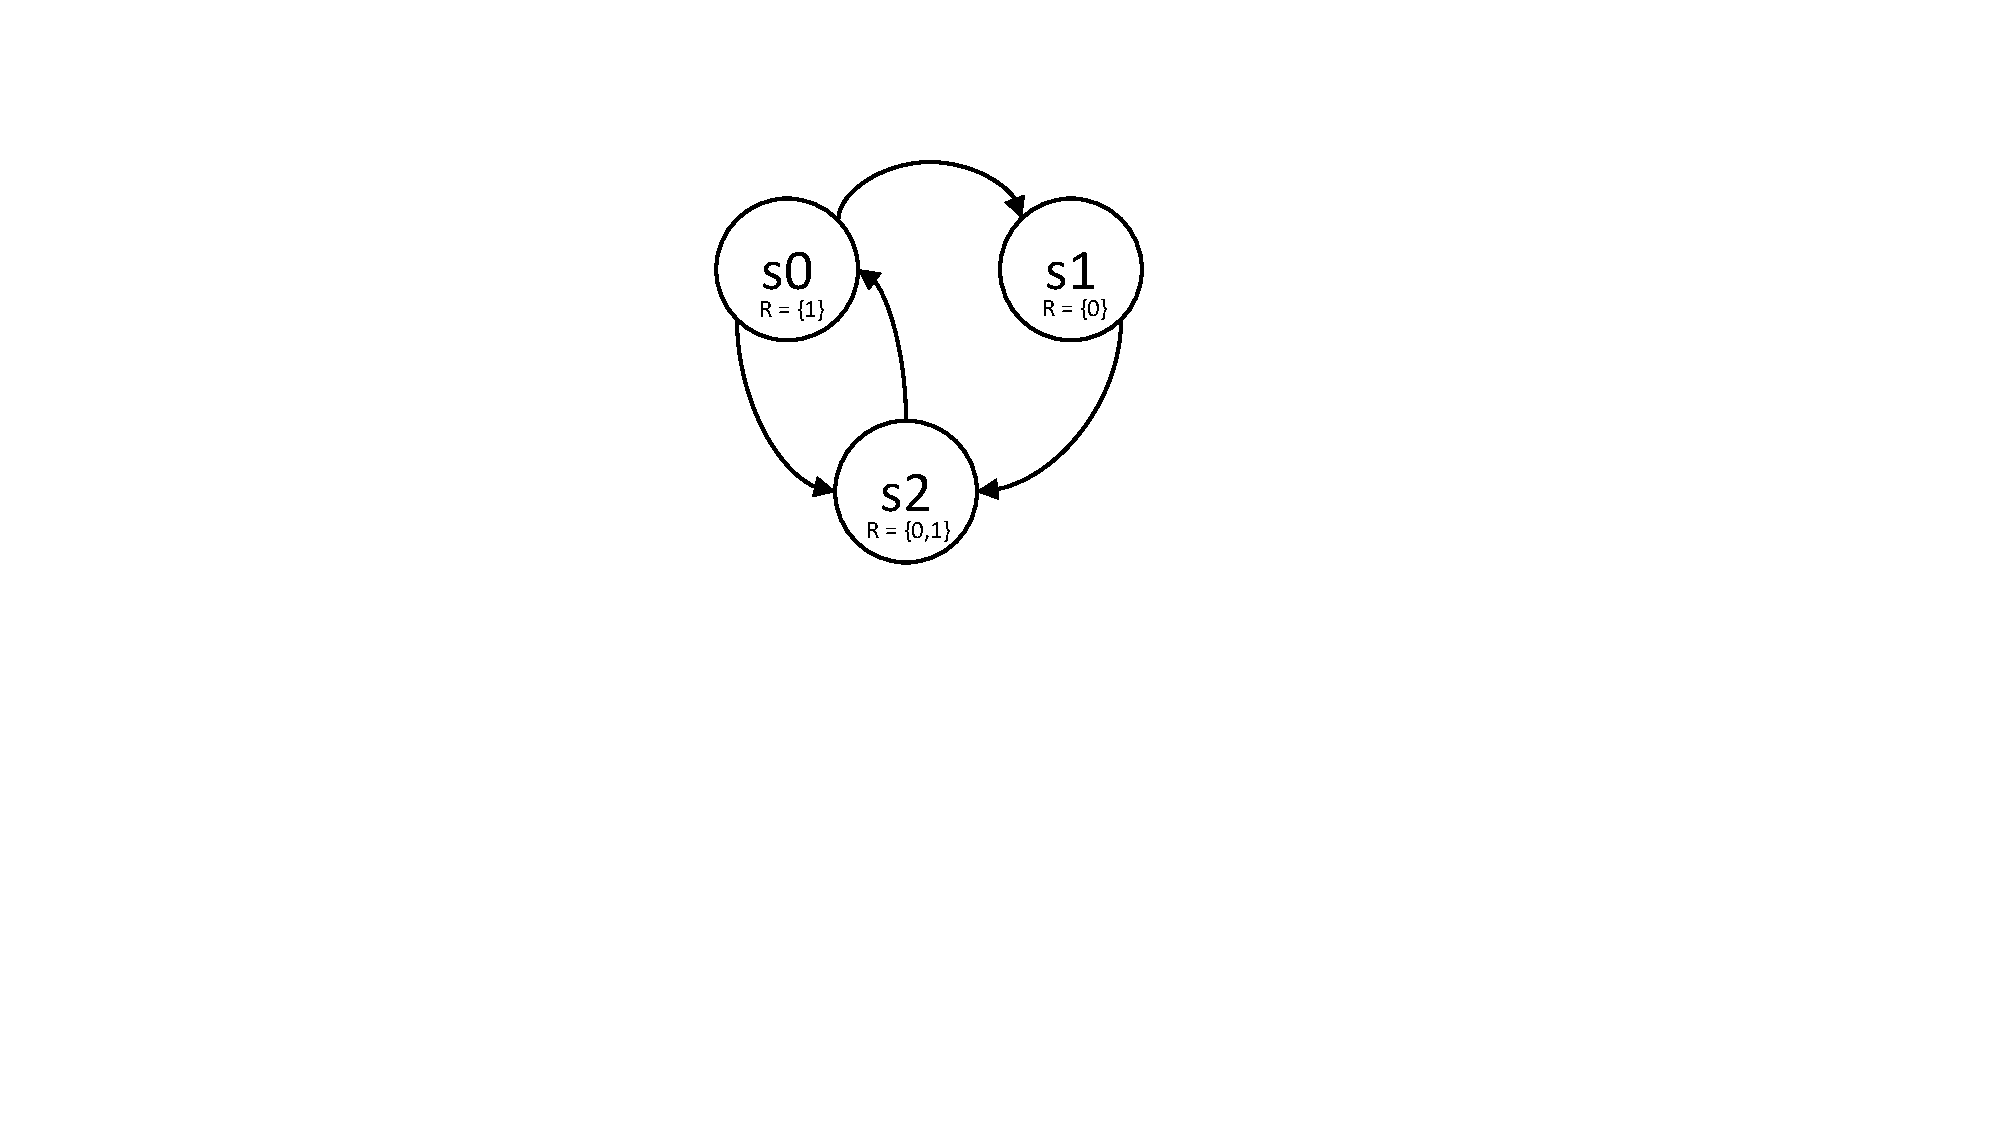
\includegraphics[width = 0.3\linewidth]{CID_graph}
	\caption{MDP Graph for my CID}
	\label{CID}
\end{figure}
\paragraph{a)} We are here discussing the transition matrix and the reward function of our process. 

The transition matrix that can be deduced from the limited length of our trace is :
\begin{equation}
	\begin{bmatrix}
		0 & p_{01} & p_{02} \\
		0 & 0 & 1 \\
		1 & 0 & 0 
	\end{bmatrix}
\end{equation}

We can see from the matrix that the process is not deterministic and rather stochastic. From state $s_0$ there is 2 possible output states $s_1$ and $s_2$. 


We also observe that the reward is not always the same when leaving a state. The first time we leave the state $s_2$ the reward is 1, as for the last step, the reward for leaving the state $s_2$ is 0. Therefore we can state the reward function is stochastic in our MDP.

\paragraph{b)}

From our trace we can compute the value of the state $s_0$. We observe the rewards after we pass in state $s_0$ and use a discount factor of $\gamma = 1$. We have then : $V(s_0) = 3 $. This is the only way to estimate a value function as we have an undefined stochastic process.

\section{Understanding of Grid Worlds}

For this part we provide in addition to the following comments, two annexes containing the optimal policy and values for my CID : 01594572, and the full code for obtaining the results of the coursework in the form of a Jupyter Notebook. 

\paragraph{1)}
My CID is 01594572, therefore we have $x=5$, $y=7$, $z=2$. As a result we have that $p=0.5$ and $\gamma=0.65$.
\paragraph{2)} We compute the optimal value function and the optimal policy by using the Value Iteration Algorithm. I used the class provided in Lab2 of this module. To the basis class, I added my own function  \texttt{optimal\_value\_policy()}, which implements the Value Iteration Algorithm. The tolerance used for the convergence of the algorithm is $0.0001$. The results can be observed in the  figure \ref{optGrid} :

\begin{figure}[H]
	\centering
	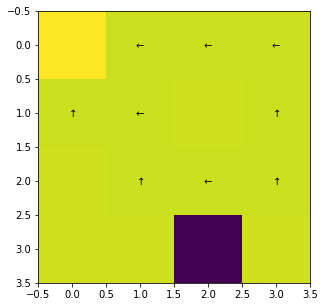
\includegraphics[width = 0.5\linewidth]{grid_optimal}
	\caption{Gridworld - Optimal Policy}
	\label{optGrid}
\end{figure}

The Optimal Value Functions for the each state are written in the following table : 
\begin{table}[H]
\centering
	\begin{tabular}{|c|c|}
		  \hline
State & Value Function \\
	  \hline
  	$s_1$ & 0 \\
	$s_2$ & 5.28 \\ 
	$s_3$ & 0.73 \\
	$s_4$ & -1.33 \\
	$s_5$& 5.91 \\
	$s_6$& 1.22 \\
	$s_7$& -2.57 \\
	$s_8$& -3.76 \\
	$s_9$& -21.65 \\
	$s_{10}$& -5.33 \\
	$s_{11}$& 0 \\
		  \hline

\end{tabular}
\end{table}


\paragraph{3)}
In state $s9$ the optimal action a is "left". The probability of this optimal action in 1 as we are in a deterministic process. But the fact that this action may not lead to the expected state in highly depending on the probability of realisation $p$. 

In our CID case we have $p=0.5$, to the probability of not leading to the expected state is $p' = (1-p) / 3$, as $p > p'$ we will more likely end in the wanted state. If $p$ gets small enough the probability wrong transition ($p'$) gets larger than $p$. If we change the value of $p$ to be small (such as $p=0.1$, see figure \ref{optGrid01}), one can observe that the optimal action is "down". At first sight this should be the worse action, but because of p, this has actually very little chance of happening.


\begin{figure}[H]
	\centering
	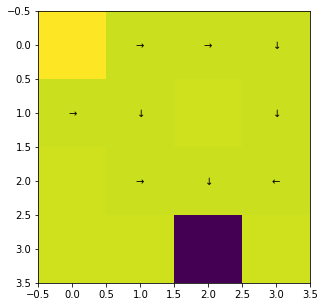
\includegraphics[width = 0.5\linewidth]{grid_p01}
	\caption{Gridworld - Optimal Policy - p = 0.1}
	\label{optGrid01}
\end{figure}


\begin{figure}[H]
	\centering
	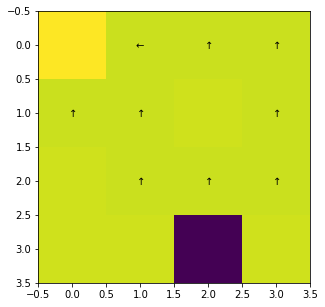
\includegraphics[width = 0.5\linewidth]{grid_g0}
	\caption{Gridworld - Optimal Policy - $\gamma$ = 0}
	\label{grid_g0}
\end{figure}

We can also discuss the influence of $\gamma$. For a small value of gamma we get a very "short-sighted" algorithm that can't see any long term rewards. If we change the discount factor to $\gamma =0$ (see figure \ref{grid_g0}) we see that the optimal action for $s_9$ is going "up", in the wall. This shows that it don't want to move from its current state, as it only sees negative rewards immediately close to it. 

\paragraph{4)}
With a global point of view for our grid world, we clearly see that influence of $p$ and $\gamma$ is really huge on the optimal values function and policy. In the case of our CID, the specific values of the parameters lead to specific behavior at certain points. For example at the state $s_6$, we can imagine that both "up" and "left" could be optimal actions. But as $p$ is not maximal, it is a safer choice to go on the left, in order to avoid the possibility of going to state $s_3$ from $s_2$. Also the value of $\gamma$ has an influence on how it values the far away rewards. The specific values of $p$ and $\gamma$ have therefore a big influence on the optimal value functions and policies. 



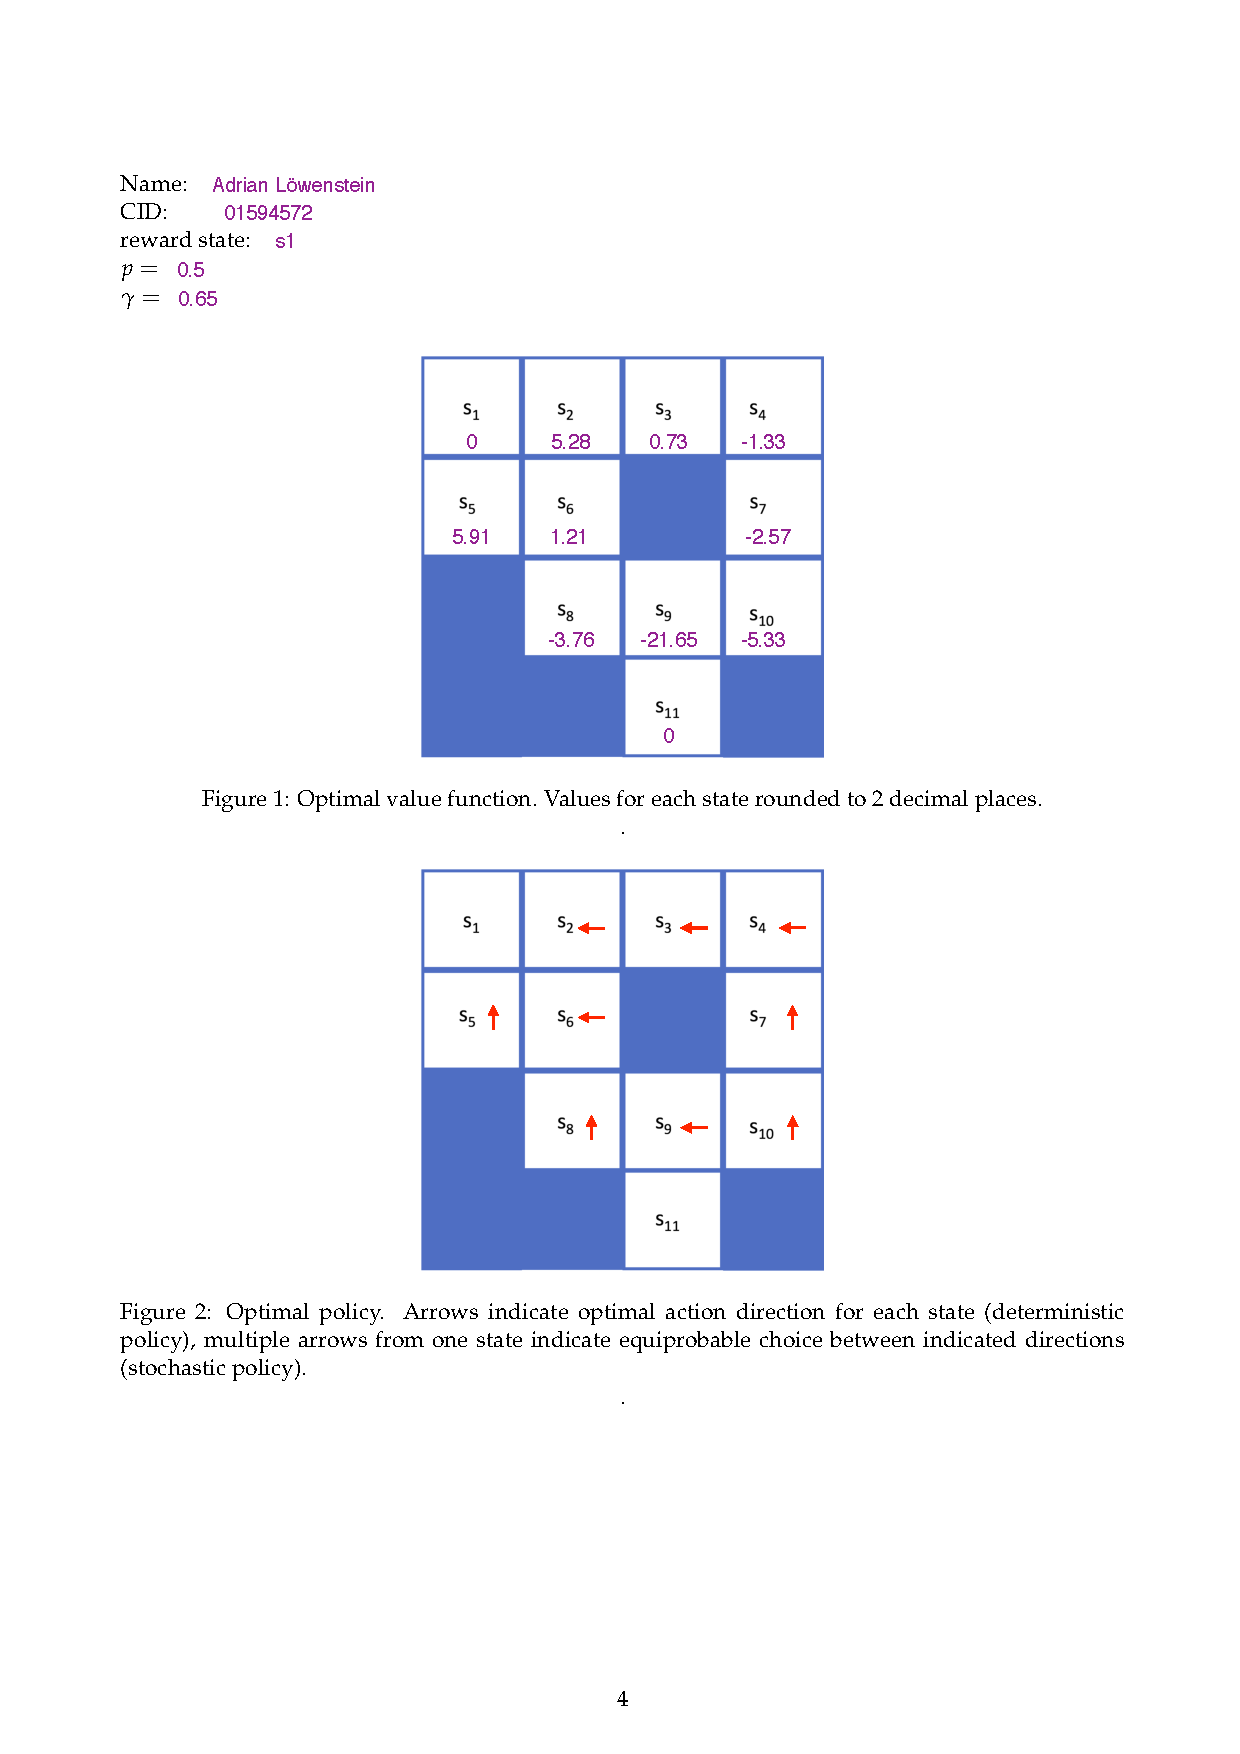
\includepdf[pages=-,offset=2cm -2cm]{gridworld}
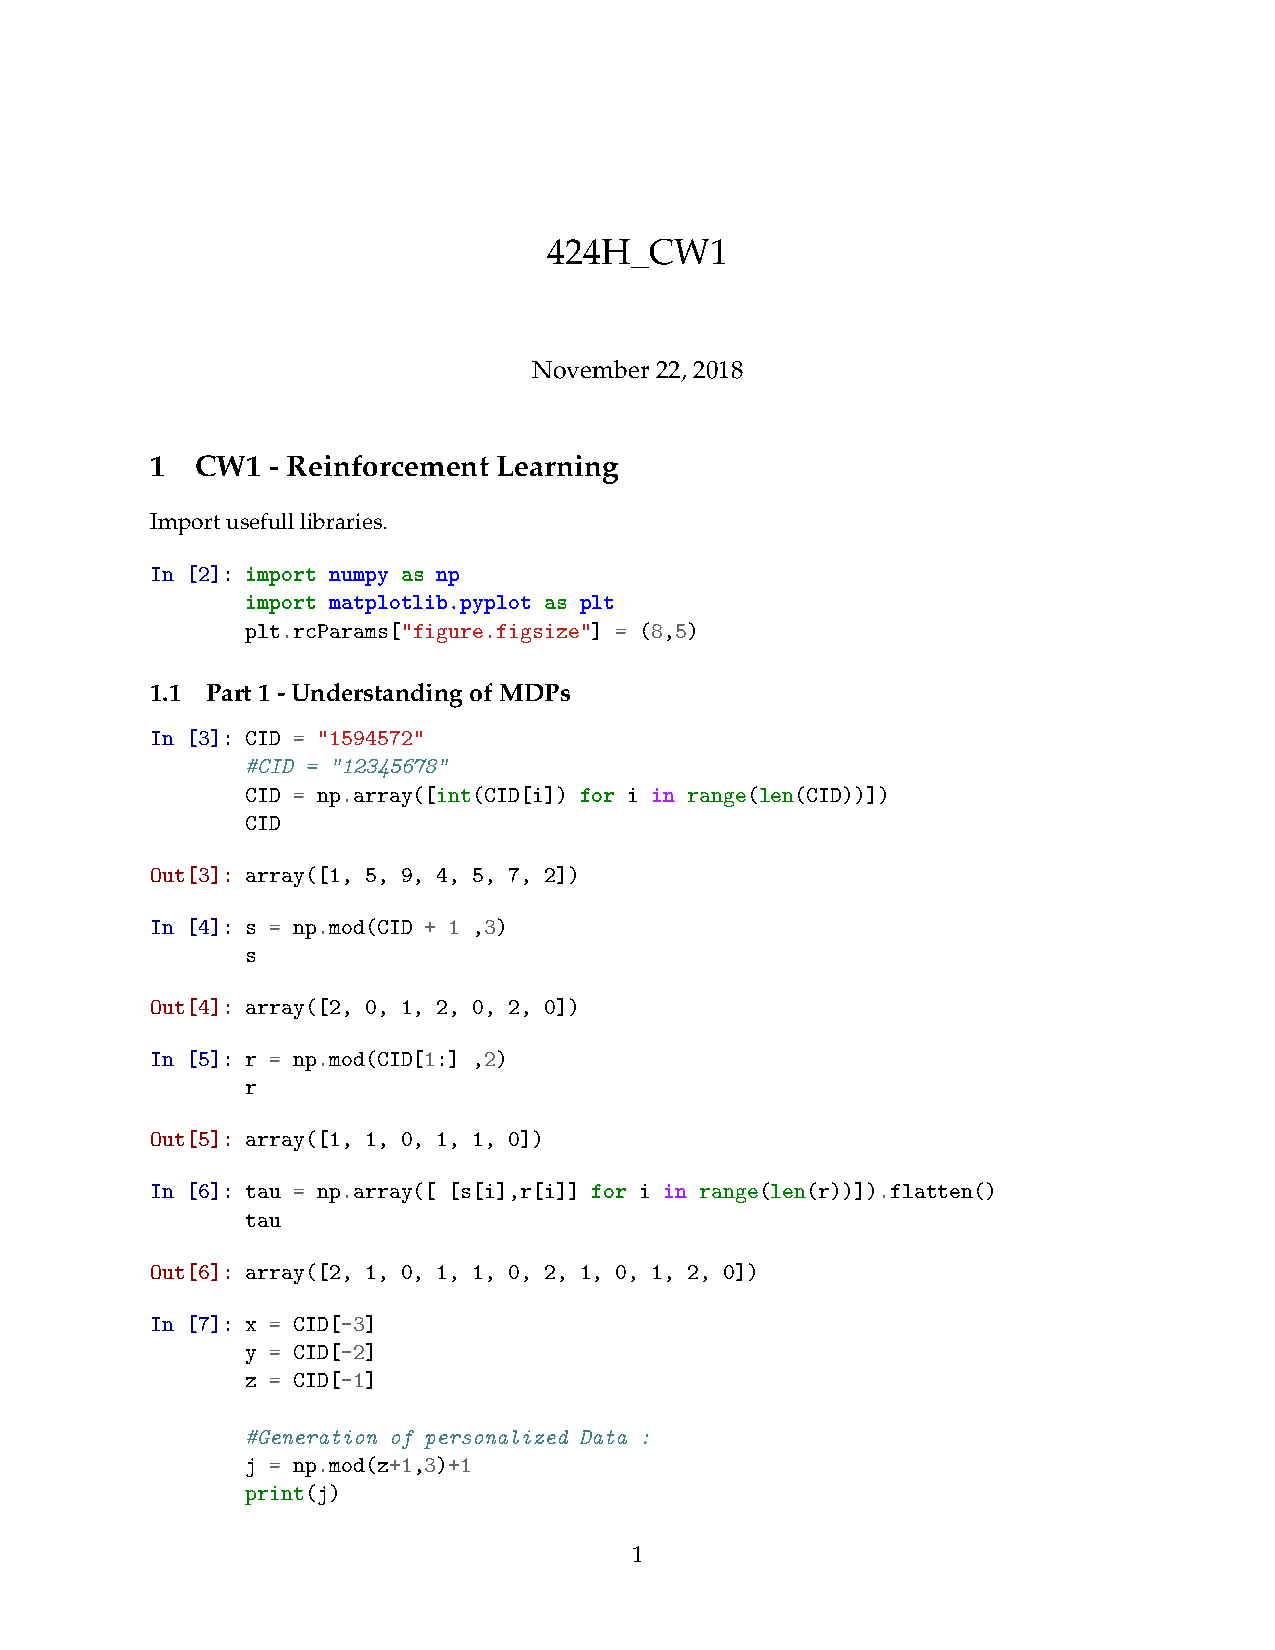
\includepdf[pages=-,offset=2cm -2cm]{424H_CW1}

\end{document}